\chapter*{Management Summary}
\addcontentsline{toc}{chapter}{Management Summary}

\section*{Die Problematik}
	F�r die Entwicklung von Applikationen wird meist eine objektorientierte Sprache wie
	Java oder C\# verwendet. Dabei sind in einem Objekt
	alle Daten und Funktionen, die f�r eine bestimmte Aufgabe notwendig sind, zusammengefasst.
	Dies erlaubt es, reelle Objekte und deren Abh�ngigkeiten einfach und strukturiert 
	in der Software abzubilden.

	Bei Datenbanken hingegen sind die Strukturelemente
	keine Objekte, sondern Tabellen, die die durch Relationen miteinander verkn�pft sind.
	Dieser Unterschied wird als ``type mismatch'' bezeichnet.
 
	Da viele Applikationen Datenbanken verwenden, muss eine M�glichkeit gefunden werden,
	diese Strukturen zu mappen. 
 	Dieses Problem ist schematisch in Abbildung \ref{fig:mgmtProblem} dargestellt.
	
	\begin{figure}[thb]
		\begin{center}
			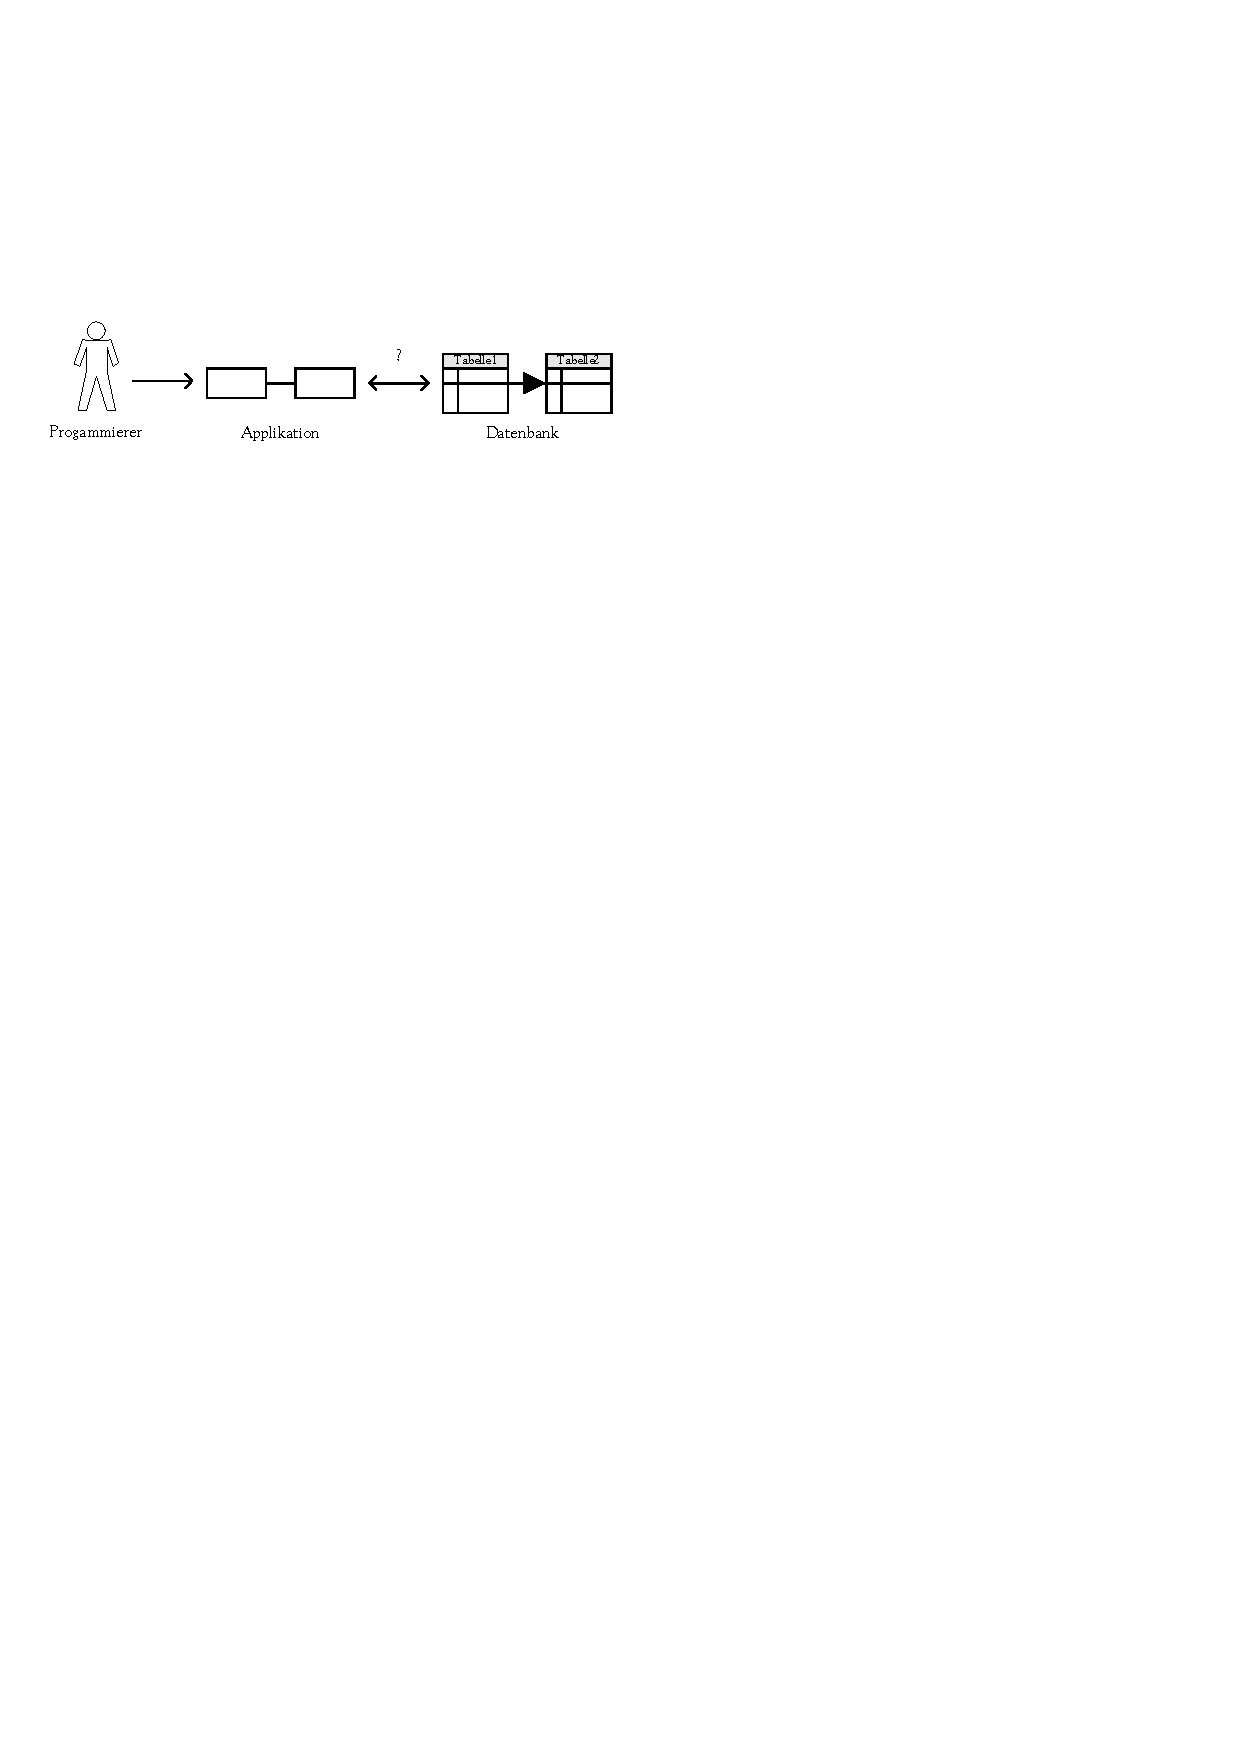
\includegraphics{./files/inc/figures/mgmtSummaryProblem}
			\caption{\label{fig:mgmtProblem}Verschiedene Strukturen bei der Applikation und der Datenbank.}
		\end{center}
	\end{figure}
 	  
\section*{Die Applikation}
	Der Name der Applikation ist \textit{S}torm 
	\textit{T}emplate-based \textit{O}bject \textit{R}elational \textit{M}apper (\textit{STORM}).
	Das Ziel von \textit{STORM} war es, ein Framework zu erstellen, das den Code f�r 
	das erw�hnte Mapping generiert. Damit wird dem Entwickler ein Teil seiner Arbeit
	abgenommen.
	
	Die Idee ist, dass der Entwickler abstrakte Domain Objekte implementiert, welche
	er mit Attributen parametrieren kann. Durch die Attributierung kann er einerseits
	das Domain Modell und andererseits das Datenbank Modell vorgeben. Anhand dieser Angaben
	wird anschliessend der gesamte Mapping Code generiert.
	Dieser Vorgang ist schematisch in Figur \ref{fig:mgmtSolution} dargestellt.
		
	
	\begin{figure}[thb]
		\begin{center}
			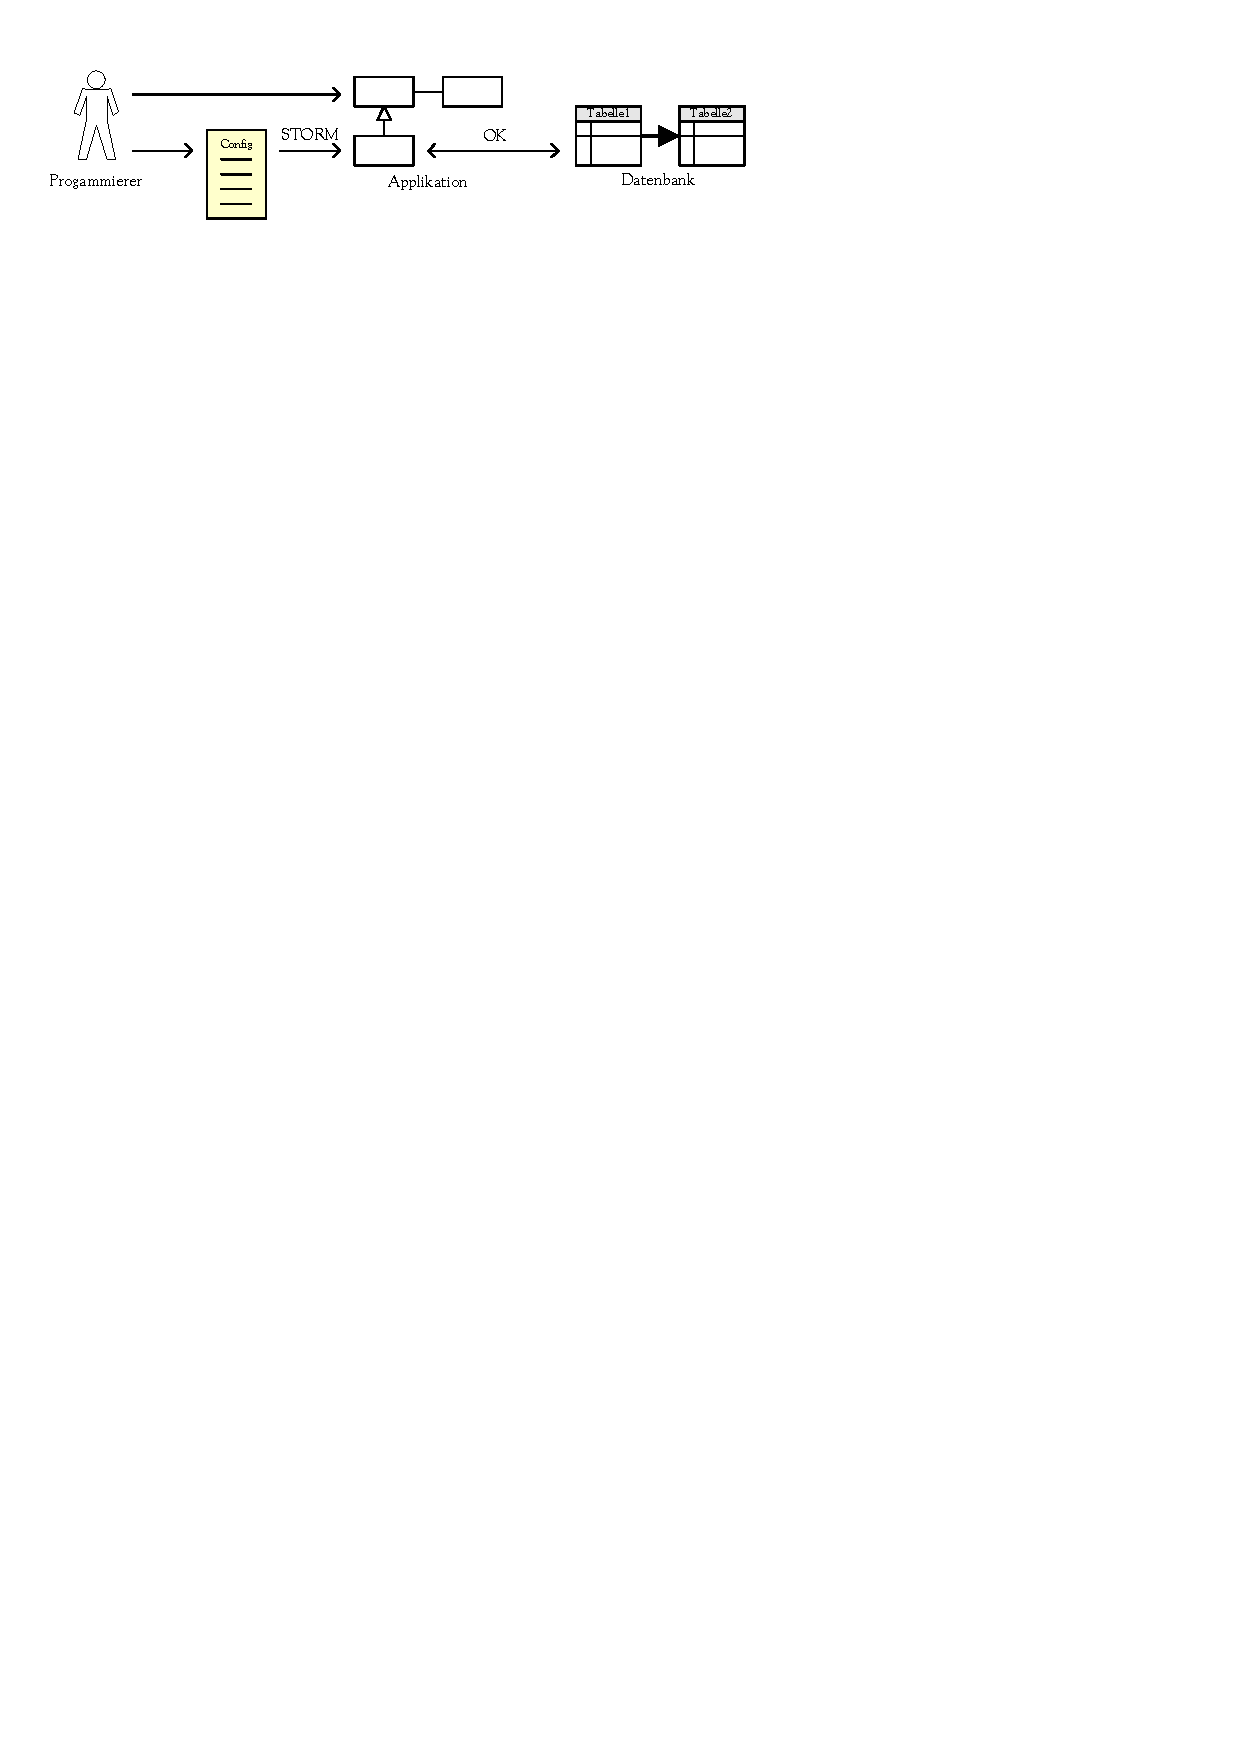
\includegraphics[width=\linewidth]{./files/inc/figures/mgmtSummarySolution}
			\caption{\label{fig:mgmtSolution}Der Code f�r das Mapping wird von \textit{STORM} erstellt. }
		\end{center}
	\end{figure}


\section*{Die Vorteile}
	Die folgende Liste gibt einen �berblick der Vorteile von \textit{STORM}.
	
	\begin{itemize}
		\item Die Entwicklungszeit einer Applikation kann stark minimiert werden.
		\item	Der generierte Mapper Code ist fehlerfrei.
		\item Der Code wird durch die Verwendung von Templates besser wartbar.
		\item Die Konfiguration wird an einem Ort, n�mlich den abstrakten Domain Objekten, vorgenommen.
		\item Der Entwickler muss sich weniger mit der Datenbank auseinandersetzen.
		\item Der Generierungsprozess ist im Visual Studio .NET eingebunden.
	\end{itemize}
	
\section*{Ausblick}
	Verschiedene Dinge konnten w�hrend dieser Arbeit nicht umgesetzt werden, da die 
	Zeit sehr begrenzt war. Daraus ergibt sich folgende Liste von Erweiterungsvorschl�gen.
		
	\begin{itemize}
		\item Meherere Locking Mechanismen werden unterst�tzt.
		\item Alle m�glichen Mapping Typen einer Datenbank werden unterst�tzt.
		\item Zus�tzlich zum Mapping zwischen Domain Objekten und Datenbank wird auch das Mapping
					zwischen Web Service Facade und Domain Objekten unterst�tzt.
		\item Als Konfigurationsm�glichkeit werden nicht nur abstrakte Klassen angeboten, sondern auch
					eine Datenbankverbindung, aus der direkt die Domain Klassen erzeugt werden.
	\end{itemize}
	
	Es w�re denkbar, die oben genannten Punkte in einer weiteren Arbeit zu implementieren. Ebenso
	m�ssten noch mehrere Testapplikationen mit \textit{STORM} entwickelt werden, um das
	Framework besser testen zu k�nnen.
	
	Die Gefahr bei der Erweiterung der jetzt bestehenden Templates ist, dass sie sehr un�bersichtlich
	werden. Man m�sste den Aufbau der Templates allenfalls �berarbeiten
	und genau planen, wie dieser aussehen m�sste, damit der Code sauber und �bersichtlich wird.
	Eine L�sung k�nnte zum Beispiel sein, ein Template in mehrere Templates aufzuteilen.
	
	Der L�sungsansatz mit den attributierten, abstrakten Klassen erscheint uns sinnvoll. 
	
	
	
	
